\begin{tikzpicture}
\begin{axis} [
     title={},
     width=\textwidth,
     height=.25\textheight,
     xlabel={\footnotesize \textbf{Task}},
     ylabel={\footnotesize \textbf{Accuracy}},
     bar width = 4pt,
     ybar = .02cm,
     xmin=0.0, xmax=10,
     ymin=0.0, ymax=90,
     x tick label style={font=\tiny},
     y tick label style={font=\tiny},
     xtick={2,4,6,8},
     xticklabels={Count (ADE), Relation (ADE), Count (COCO), Relation (COCO)},
     y label style={at={(axis description cs:0.05,.5)},anchor=south},
     ymajorgrids=false,
     xmajorgrids=false,
     legend style={
			at={(0.5,-0.35)},
			anchor=north,
			legend columns=3,
            }
] 

\addplot[color=blue!40, fill=blue, area legend] coordinates{(2, 24.6) (4, 51.2) (6, 42.8) (8, 53.2)};
\addplot[color=blue!40, fill=blue!40,  area legend] coordinates {(2, 5.8) (4, 4.1) (6, 4.9) (8, 2.2)};
%\addplot[color=blue!40, fill=blue!40,  area legend] coordinates {(2, 0) (4, 0) (6, 0) (8, 0)};
%\addplot[color=blue!40, fill=blue!20,  area legend] coordinates {(2, 0) (4, 0) (6, 0) (8, 0)};
\addplot[color=blue!40, fill=blue!20,  area legend] coordinates {(2, 35.3) (4, 60.1) (6, 59.4) (8, 65.2)};

\addplot[color=red!20, fill=red!20,  area legend] coordinates {(2, 48.0) (4, 64.6) (6, 66.8) (8, 71.0)};
\addplot[color=red!60, fill=red!60,  area legend] coordinates {(2, 43.6) (4, 68.4) (6, 62.3) (8, 73.8)};
\addplot[color=red, fill=red,  area legend] coordinates {(2 , 51.8) (4, 80.8) (6, 75.1) (8, 84.7)};

\legend{\textbf{OMG-Llava (7B)}, \textbf{Llava-G (7B)}, \textbf{GLaMM$\dagger$ (7B)}, \textbf{Llava (13B)}, \textbf{Llava (7B)}, \textbf{Cambrian (8B)}}

\end{axis}
\end{tikzpicture}